% CS336 assignment 讲义版式：letter + CM + 蓝/橙框
\newcommand{\reporoot}{../..}

\usepackage{lmodern}
\usepackage{amsmath,amssymb,bm}
\usepackage[letterpaper,margin=1in]{geometry}
\usepackage{xcolor}
\usepackage{booktabs}
\usepackage{caption}
\captionsetup{font=small, labelfont=bf, skip=4pt}
\usepackage{tikz}
\usetikzlibrary{arrows.meta,positioning,calc}
\usepackage{enumitem}
\usepackage{listings}
\usepackage{setspace}
\usepackage[most]{tcolorbox}
\usepackage{titlesec}
\usepackage{fancyhdr}
\usepackage{hyperref}

\definecolor{csblue}{RGB}{0,112,192}
\definecolor{csorange}{RGB}{230,126,34}
\definecolor{csteal}{RGB}{0,128,128}
\definecolor{csstring}{RGB}{46,139,87}
\colorlet{structurecolor}{csblue}
\colorlet{second}{csorange}

\hypersetup{
  colorlinks=true,
  linkcolor=red!70!black,
  urlcolor=csblue,
  citecolor=red!70!black,
  breaklinks=true,
  linktoc=all,
}
\setcounter{tocdepth}{2}

\IfFontExistsTF{DejaVu Sans Mono}{
  \setmonofont{DejaVu Sans Mono}[Scale=0.88]
}{}

\setlength{\parindent}{0pt}
\setlength{\parskip}{0.55em}
\setstretch{1.12}
\setlist{nosep, leftmargin=1.35em, itemsep=0.2em, topsep=0.35em}
\setlist[enumerate,1]{label=\arabic*.}
\setlist[itemize,1]{label=\textbullet}

\titleformat{\section}{\large\bfseries}{\thesection}{0.55em}{}
\titleformat{\subsection}{\normalsize\bfseries}{\thesubsection}{0.45em}{}
\titleformat{\subsubsection}{\normalsize\bfseries}{\thesubsubsection}{0.4em}{}
\titlespacing*{\section}{0pt}{1.35em}{0.4em}
\titlespacing*{\subsection}{0pt}{1.05em}{0.3em}
\titlespacing*{\subsubsection}{0pt}{0.85em}{0.25em}

\pagestyle{plain}
\fancyhf{}
\renewcommand{\headrulewidth}{0pt}
\cfoot{\thepage}

% 蓝框 = CS336 Low-Resource Tip；橙框 = Problem
\newcommand{\csboxline}{%
  \par\vspace{3pt}%
  \noindent{\color{black}\rule{\linewidth}{0.45pt}}\par
  \vspace{6pt}%
}
\newtcolorbox{csframe}[1]{
  colback=white,
  colframe=#1,
  boxrule=0.7pt,
  sharp corners,
  left=8pt, right=8pt, top=6pt, bottom=7pt,
  before skip=10pt, after skip=10pt,
}
\newenvironment{tipbox}[1]{%
  \begin{csframe}{csblue}%
  \noindent\textbf{#1}\csboxline
}{\end{csframe}}
\newenvironment{problembox}[1]{%
  \begin{csframe}{csorange}%
  \noindent\textbf{#1}\csboxline
}{\end{csframe}}

% 旧章命令映射到 article 节（正文仍写 \chapter / \section）
\let\textbooksection\section
\let\textbooksubsection\subsection
\NewDocumentCommand{\chapter}{s m}{%
  \IfBooleanTF{#1}{\textbooksection*{#2}}{\textbooksection{#2}}%
}
\RenewDocumentCommand{\section}{s m}{%
  \IfBooleanTF{#1}{\textbooksubsection*{#2}}{\textbooksubsection{#2}}%
}
\renewcommand{\subsection}{\subsubsection}
\renewcommand{\part}[1]{}
\providecommand{\frontmatter}{}
\providecommand{\mainmatter}{}
\renewcommand{\maketitle}{}

\newenvironment{introduction}{%
  \par\noindent\textbf{本讲要点}%
  \begin{itemize}%
}{\end{itemize}}
\newenvironment{note}{\begin{tipbox}{Note}}{\end{tipbox}}
\newenvironment{remark}{\begin{tipbox}{Remark}}{\end{tipbox}}
\newenvironment{conclusion}{\begin{tipbox}{Conclusion}}{\end{tipbox}}
\newenvironment{proposition}[1]{\begin{tipbox}{#1}}{\end{tipbox}}
\newenvironment{definition}[1]{\begin{tipbox}{#1}}{\end{tipbox}}
\newenvironment{runcmd}[1][怎么跑]{\begin{tipbox}{#1}}{\end{tipbox}}
\newenvironment{exercise}[1][]{\begin{problembox}{Problem#1}}{\end{problembox}}
\newenvironment{problemset}[1][]{%
  \begin{problembox}{#1}%
  \begin{enumerate}[label=(\alph*)]%
}{%
  \end{enumerate}%
  \end{problembox}%
}

\renewcommand{\arraystretch}{1.15}

\lstdefinestyle{pythoncode}{
  language=Python,
  basicstyle=\ttfamily\small,
  keywordstyle=\color{csteal},
  commentstyle=\color{black!45},
  stringstyle=\color{csstring},
  showstringspaces=false,
  breaklines=true,
  frame=none,
  numbers=none,
  tabsize=4,
  captionpos=b,
  columns=flexible,
  keepspaces=true,
  showlines=false,
  xleftmargin=0.6em,
}
\lstdefinestyle{shell}{
  language=Python,
  basicstyle=\ttfamily\small,
  keywordstyle=\color{csteal},
  commentstyle=\color{black!45},
  stringstyle=\color{csstring},
  breaklines=true,
  frame=none,
  numbers=none,
  columns=flexible,
  keepspaces=true,
  xleftmargin=0.6em,
}
\lstset{style=pythoncode}

\newcommand{\src}[4]{%
  \lstinputlisting[
    style=pythoncode,
    firstline=#2,
    lastline=#3,
    caption={#4},
  ]{\reporoot/#1}%
  \par\vspace{-0.3em}\noindent{\small 文件：\texttt{\detokenize{#1}:#2--#3}}%
}

\newcommand{\run}[1]{\texttt{\detokenize{#1}}}
\newcommand{\pyfile}[1]{\texttt{\detokenize{#1}}}
\providecommand{\kaishu}{}

\tikzset{
  opbox/.style={draw=csblue, thick, fill=csblue!8, inner sep=4pt, font=\small, align=center},
  sram/.style={draw=csorange, thick, fill=csorange!12, inner sep=4pt, font=\small, align=center},
  hbm/.style={draw=black!45, thick, fill=black!4, inner sep=4pt, font=\small, align=center},
  arr/.style={-Latex, csblue, thick},
  arrd/.style={-Latex, csorange, thick},
}
\newcommand{\fignote}[1]{\par\vspace{3pt}{\centering\small #1\par}\vspace{4pt}}
\graphicspath{{figures/}}
\newcommand{\facite}{Dao. \emph{FlashAttention-2: Faster Attention with Better Parallelism and Work Partitioning}. ICLR 2024}
\newcommand{\faurl}{https://arxiv.org/abs/2307.08691}
\newcommand{\paperfig}[3]{%
\begin{center}
\includegraphics[width=#2\linewidth]{#1}%
\fignote{#3}
\end{center}}
% 算子数据流图。先图后码。

\newcommand{\figmemhier}{%
\begin{center}
\begin{tikzpicture}[font=\small, node distance=0.7cm]
  \node[hbm, minimum width=7.2cm] (hbm) {HBM：大、慢。张量 $Q,K,V,O$ 住这里};
  \node[sram, minimum width=7.2cm, below=of hbm] (sram) {SRAM / 寄存器：小、快。tile 与 $(m,\ell)$ 住这里};
  \node[opbox, minimum width=7.2cm, below=of sram] (alu) {Tensor Core / ALU：\texttt{tl.dot}、\texttt{tl.sum}};
  \draw[arr] (hbm) -- (sram) node[midway, right=2pt] {load / store};
  \draw[arr] (sram) -- (alu);
\end{tikzpicture}
\fignote{换核改的是 HBM 往返和片上驻留，不是 Transformer 公式。}
\end{center}}

\newcommand{\figgpuhier}{%
\begin{center}
\begin{tikzpicture}[font=\small, node distance=0.5cm]
  \node[hbm, minimum width=8.6cm] (hbm) {HBM：整卡一份，张量住这里，往返最贵};
  \node[opbox, minimum width=8.6cm, below=of hbm] (l2) {L2：全芯片共享缓存};
  \node[sram, minimum width=8.6cm, below=of l2] (sm) {许多 SM：各有 SRAM（shared memory）、寄存器、Tensor Core};
  \node[opbox, minimum width=8.6cm, below=of sm] (wp) {一个 SM 上：硬件按 warp（32 线程、SIMT 锁步）调度};
  \draw[arr] (hbm) -- (l2);
  \draw[arr] (l2) -- (sm);
  \draw[arr] (sm) -- (wp);
\end{tikzpicture}
\fignote{一块 GPU $=$ 慢而大的 HBM $+$ 许多能独立干活的 SM。算子优化就是少碰 HBM、让 tile 留在 SM 上。}
\end{center}}

\newcommand{\figcudagrid}{%
\begin{center}
\begin{tikzpicture}[x=0.78cm,y=0.62cm,font=\small]
  \foreach \j in {0,1,2} {
    \draw[csblue, thick, fill=csblue!8] (\j*3.55, 0) rectangle ++(3.3, 2.35);
    \node at (\j*3.55+1.65, 2.0) {block \j};
    \foreach \t in {0,1,2,3} {
      \fill[csorange!40] (\j*3.55+0.22+\t*0.76, 0.28) rectangle ++(0.66, 0.85);
    }
    \node[font=\footnotesize] at (\j*3.55+1.65, 0.68) {threads};
  }
  \draw[csblue, thick] (-0.25,-0.45) rectangle (10.45,2.7);
  \node at (5.1, 3.15) {一次 \texttt{kernel<<<grid,block>>>} $=$ 一个 grid};
\end{tikzpicture}
\fignote{每个 block 落到一个 SM，块内线程共享 SRAM。CUDA 要你写「第 $t$ 号线程做什么」。}
\end{center}}

\newcommand{\figtritonabs}{%
\begin{center}
\begin{tikzpicture}[font=\small]
  \node[hbm, minimum width=4.3cm] (c) {CUDA：thread / warp};
  \node[opbox, minimum width=4.3cm, right=1.2cm of c] (t) {Triton：program $\approx$ block};
  \draw[arr] (c) -- (t);
\end{tikzpicture}
\fignote{编译器把 tile 摊到 warp。grid 和怎么分块仍要你定。}
\end{center}}

\newcommand{\figpidone}{%
\begin{center}
\begin{tikzpicture}[x=0.85cm,y=0.7cm,font=\small]
  \draw[csblue, thick] (0,0) rectangle (9,1.15);
  \draw[csblue] (3,0) -- (3,1.15);
  \draw[csblue] (6,0) -- (6,1.15);
  \fill[csblue!15] (0,0) rectangle (3,1.15);
  \node at (1.5,0.58) {block 0};
  \node at (4.5,0.58) {block 1};
  \node at (7.5,0.58) {block 2};
  \node[csblue] at (1.5,-0.4) {\texttt{pid}=0};
  \node[csblue] at (4.5,-0.4) {\texttt{pid}=1};
  \node[csblue] at (7.5,-0.4) {\texttt{pid}=2};
  \node at (4.5,1.6) {数组 $[0,\ldots,n-1]$};
\end{tikzpicture}
\fignote{一份 program 吃一块 \texttt{BLOCK}；尾巴用 \texttt{mask}。}
\end{center}}

\newcommand{\figtiletwo}{%
\begin{center}
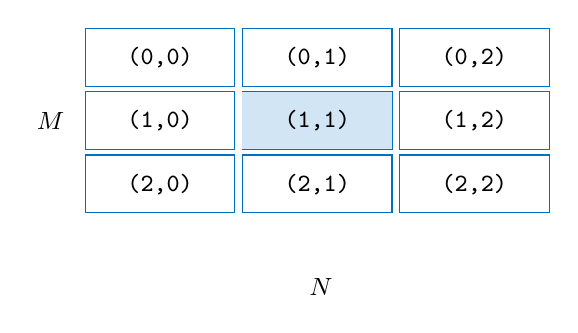
\begin{tikzpicture}[x=0.95cm,y=0.7cm,font=\small]
  \foreach \i in {0,1,2} {
    \foreach \j in {0,1,2} {
      \draw[csblue] (\j*2.1, -\i*1.15) rectangle ++(2.0,1.05);
      \node at (\j*2.1+1.0, -\i*1.15+0.52) {\texttt{(\i,\j)}};
    }
  }
  \fill[csblue!18] (2.1, -1.15) rectangle ++(2.0,1.05);
  \node at (3.1, -0.63) {\texttt{(1,1)}};
  \node[left] at (-0.15, -1.15+0.52) {$M$};
  \node at (3.15, -3.65) {$N$};
\end{tikzpicture}
\fignote{二维：\texttt{pid\_m} 管行块，\texttt{pid\_n} 管列块，各自乘 stride。}
\end{center}}

\newcommand{\figbandwidth}{%
\begin{center}
\begin{tikzpicture}[font=\small, node distance=1.15cm]
  \node[hbm] (x) {$x$};
  \node[hbm, right=of x] (y) {$y$};
  \node[sram, below=1.2cm of {$(x)!0.5!(y)$}] (alu) {$x+y$ 在片上};
  \node[hbm, below=of alu] (o) {out};
  \draw[arr] (x) -- (alu);
  \draw[arr] (y) -- (alu);
  \draw[arr] (alu) -- (o);
\end{tikzpicture}
\fignote{带宽绑定：一次加法，时间看两次 load、一次 store。}
\end{center}}

\newcommand{\figswiglu}{%
\begin{center}
\begin{tikzpicture}[font=\footnotesize, node distance=0.55cm]
  \node[align=center] at (2.2, 3.15) {\textbf{浅：中间 $a,b$ 进 HBM}};
  \node[hbm] (x1) at (0,2.2) {$x$};
  \node[hbm] (a1) at (2.0,2.55) {$a{=}xW_1$};
  \node[hbm] (b1) at (2.0,1.85) {$b{=}xW_2$};
  \node[hbm] (o1) at (4.4,2.2) {$\mathrm{SiLU}(a)\odot b$};
  \draw[arr] (x1) -- (a1);
  \draw[arr] (x1) -- (b1);
  \draw[arr] (a1) -- (o1);
  \draw[arr] (b1) -- (o1);
  \draw[dotted] (5.5,-0.15) -- (5.5,3.25);
  \node[align=center] at (8.6, 3.15) {\textbf{深：沿 $K$ 两次 dot}};
  \node[hbm] (x2) at (6.5,2.2) {$x$};
  \node[sram] (t2) at (8.6,2.2) {tile 上 $a,b$};
  \node[hbm] (o2) at (10.7,2.2) {out};
  \draw[arr] (x2) -- (t2);
  \draw[arr] (t2) -- (o2);
\end{tikzpicture}
\fignote{深融合少两次中间 GEMM 的 HBM 往返；大矩阵仍可能慢于 cuBLAS。}
\end{center}}

\newcommand{\figmatmul}{%
\begin{center}
\begin{tikzpicture}[x=0.48cm,y=0.48cm,font=\small]
  \draw[black!45, thick, fill=black!4] (0,1.6) rectangle (5.2,8.2);
  \fill[csblue!28] (0,4.4) rectangle (5.2,6.2);
  \node at (2.6,8.75) {$A$ $(M{\times}K)$};
  \node at (2.6,5.3) {$A_{ik}$};
  \draw[black!45, thick, fill=black!4] (7.2,5.6) rectangle (15.2,8.2);
  \fill[csblue!28] (9.6,5.6) rectangle (11.6,8.2);
  \node at (11.2,8.75) {$B$ $(K{\times}N)$};
  \node at (10.6,6.9) {$B_{kj}$};
  \draw[csorange, thick, fill=csorange!22] (9.6,1.8) rectangle (11.6,3.8);
  \node at (10.6,2.8) {$C_{ij}$};
  \draw[arr] (5.2,5.3) -- (9.55,3.1);
  \draw[arrd] (10.6,5.55) -- (10.6,3.9);
  \node[font=\footnotesize] at (7.6,4.15) {$\sum_k$};
  \node[font=\footnotesize] at (10.6,1.25) {SRAM 累加，沿 $K$ 循环};
\end{tikzpicture}
\fignote{一个 program 只写一块 $C$；归约维 $K$ 必须在核内 \texttt{for}，不能拆成不同 pid。}
\end{center}}

\newcommand{\figsoftmax}{%
\begin{center}
\begin{tikzpicture}[x=0.55cm,y=0.55cm,font=\small]
  \node at (4, 5.1) {\textbf{对：一行一个 pid}};
  \foreach \r in {0,1,2} {
    \draw[csblue] (0, 4-\r) rectangle (8, 4.85-\r);
    \fill[csblue!20] (0, 4-\r) rectangle (8, 4.85-\r);
    \node at (-1.15, 4.4-\r) {\texttt{pid}=\r};
    \node at (4, 4.4-\r) {$\max$ / $\mathrm{sum}$ 整行};
  }
  \begin{scope}[shift={(10.2,0)}]
    \node at (3.2, 5.1) {\textbf{错：把归约维切开}};
    \foreach \c in {0,1,2} {
      \draw[csorange] (\c*2.1, 2.2) rectangle ++(2.0, 2.5);
      \node at (\c*2.1+1.0, 3.45) {\texttt{pid}=\c};
    }
    \node[csorange, font=\footnotesize, align=center] at (3.15, 1.55) {各块的 max\\无法再合并};
  \end{scope}
\end{tikzpicture}
\fignote{归约维留下给核内 \texttt{for}；pid 只切独立的行（或 batch）。}
\end{center}}

\newcommand{\figonline}{%
\begin{center}
\begin{tikzpicture}[font=\small, node distance=0.85cm]
  \node[hbm] (x) {$x$ 一行};
  \node[sram, right=1.3cm of x] (s) {$(m,d)$};
  \node[hbm, right=1.3cm of s] (y) {$y$};
  \draw[arr] (x) -- node[above, font=\footnotesize] {第 1 趟} (s);
  \draw[arr] (s) -- node[above, font=\footnotesize] {第 2 趟} (y);
  \node[below=0.35cm of s, font=\footnotesize, align=center]
    {$m'=\max(m,m_{\mathrm{blk}})$\\$d'=d\,e^{m-m'}+d_{\mathrm{blk}}e^{m_{\mathrm{blk}}-m'}$};
\end{tikzpicture}
\fignote{online 统计量可合并，所以 Flash 能把 $K/V$ 留在内层循环。}
\end{center}}

\newcommand{\fignorm}{%
\begin{center}
\begin{tikzpicture}[x=0.5cm,y=0.5cm,font=\small]
  \foreach \r in {0,1,2} {
    \draw[csblue] (0, 3.2-\r*1.15) rectangle (7, 4.15-\r*1.15);
    \fill[csblue!12] (0, 3.2-\r*1.15) rectangle (7, 4.15-\r*1.15);
    \node at (3.5, 3.65-\r*1.15) {行 \r：$(\mu,\sigma)$ 本地};
  }
  \draw[csorange, thick] (8.2, 0.9) rectangle (13.4, 2.0);
  \node at (10.8, 1.45) {$\mathrm{d}\gamma,\mathrm{d}\beta$};
  \draw[arrd] (7.1, 3.65) -- (8.2, 1.7);
  \draw[arrd] (7.1, 2.5) -- (8.2, 1.55);
  \draw[arrd] (7.1, 1.35) -- (8.2, 1.4);
  \node[font=\footnotesize, align=left] at (10.8, 0.25) {\texttt{atomic\_add}};
\end{tikzpicture}
\fignote{$\mathrm{d}x$ 按行写；$\mathrm{d}\gamma/\mathrm{d}\beta$ 形状是 $(N,)$，多行必须原子加。}
\end{center}}

\newcommand{\fignaiveattn}{%
\begin{center}
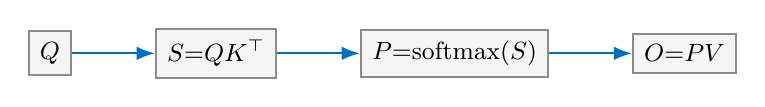
\begin{tikzpicture}[font=\small, node distance=1.05cm]
  \node[hbm] (q) {$Q$};
  \node[hbm, right=of q] (s) {$S{=}QK^\top$};
  \node[hbm, right=of s] (p) {$P{=}\mathrm{softmax}(S)$};
  \node[hbm, right=of p] (o) {$O{=}PV$};
  \draw[arr] (q) -- (s);
  \draw[arr] (s) -- (p);
  \draw[arr] (p) -- (o);
\end{tikzpicture}
\fignote{Naive：$S,P$ 是 $(S,S)$，写进 HBM。多头若 Host 串 launch，不是融合。}
\end{center}}

\newcommand{\figflashloop}{%
\begin{center}
\begin{tikzpicture}[x=1.05cm,y=0.78cm,font=\small]
  \foreach \j in {0,1,2,3} {\node at (\j+0.5, 3.55) {$K_{\j}$};}
  \foreach \i in {0,1,2} {
    \node at (-0.55, 2.45-\i) {$Q_{\i}$};
    \foreach \j in {0,1,2,3} {
      \fill[black!5] (\j, 2-\i) rectangle ++(0.95,0.85);
      \draw[black!40] (\j, 2-\i) rectangle ++(0.95,0.85);
    }
  }
  \fill[csorange!40] (0,1) rectangle ++(0.95,0.85);
  \fill[csorange!40] (1,1) rectangle ++(0.95,0.85);
  \draw[csorange, thick] (0,1) rectangle ++(0.95,0.85);
  \draw[csorange, thick] (1,1) rectangle ++(0.95,0.85);
  \node[sram, anchor=west, align=left] at (4.35, 1.42)
    {当前 $Q_1$\\SRAM $(m,\ell,\mathrm{acc})$\\没有 $S/P$};
  \node[font=\footnotesize] at (2.0, -0.35) {橙：内层正在扫的 $K$ 块};
\end{tikzpicture}
\fignote{Flash 双循环：外 $Q$ 可映射成 pid，内 $K/V$ 必须在同一 program 里扫。}
\end{center}}

\newcommand{\figcausal}{%
\begin{center}
\begin{tikzpicture}[x=0.48cm,y=0.48cm,font=\small]
  \foreach \i in {0,...,4} {
    \foreach \j in {0,...,4} {
      \ifnum\j>\i
        \fill[black!14] (\j, 5-\i) rectangle ++(1,1);
      \else
        \fill[csblue!40] (\j, 5-\i) rectangle ++(1,1);
      \fi
      \draw[black!35] (\j, 5-\i) rectangle ++(1,1);
    }
  }
  \draw[csorange, very thick] (1,3) rectangle (3,5);
  \node at (2.5, -0.45) {$K$ 列 $n$};
  \node[rotate=90] at (-0.65, 2.5) {$Q$ 行 $m$};
  \node[font=\footnotesize, align=left] at (8.9, 3.35)
    {蓝：$\texttt{offs\_n}\le\texttt{offs\_m}$\\灰：$-\infty$\\橙框：一块 $K$ 同时含过去和未来\\打在 \texttt{qk} 上，不是 load mask};
\end{tikzpicture}
\fignote{一块 $K$ 里常常同时有过去和未来，不能靠越界 mask 代替 causal。}
\end{center}}

\newcommand{\figfagrid}{%
\begin{center}
\begin{tikzpicture}[font=\small, node distance=0.35cm]
  \node[opbox, minimum width=5.4cm] (t) {教学：\texttt{grid=(B,H)}\\一个 program 扫完该头全部 $Q$};
  \node[sram, minimum width=5.4cm, below=0.7cm of t] (f) {加速：\texttt{grid=($S/B_M$, B, H)}\\一块 $Q$ 一个 program};
  \draw[arrd] (t) -- (f);
\end{tikzpicture}
\fignote{先读懂教学版的双循环，再看 Q 块并行和 GQA 的 \texttt{GROUP}。}
\end{center}}

\newcommand{\figlaunch}{%
\begin{center}
\begin{tikzpicture}[font=\small, node distance=0.45cm]
  \node[hbm, minimum width=5.6cm] (bad) {Host \texttt{for h}：每个头一次 launch};
  \node[opbox, minimum width=5.6cm, below=0.65cm of bad] (ok) {\texttt{grid=(B,H)}：一次 launch，$B{\times}H$ 个 program};
  \draw[arrd] (bad) -- (ok);
\end{tikzpicture}
\fignote{nsys 先数 kernel 名字和次数。Python 循环调核，时间线会被切碎。}
\end{center}}

\newcommand{\figtrainops}{%
\begin{center}
\begin{tikzpicture}[font=\small]
  \node[opbox, minimum width=6.4cm] (d) {默认 \texttt{fa}：只换注意力};
  \node[hbm, minimum width=6.4cm, below=0.7cm of d] (t) {对照 \texttt{fa,ln,swiglu}：教学 GEMM 常负优化};
  \draw[arr] (d) -- (t);
\end{tikzpicture}
\fignote{训练图里能换核，不等于该把所有层都换成教学实现。}
\end{center}}

\newcommand{\figgqa}{%
\begin{center}
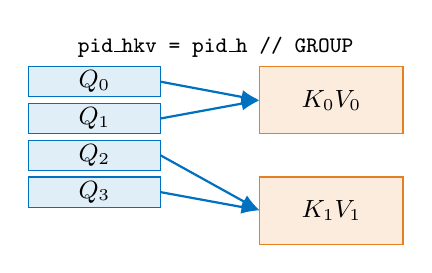
\begin{tikzpicture}[x=0.7cm,y=0.55cm,font=\small]
  \foreach \i in {0,1,2,3} {
    \draw[csblue, fill=csblue!12] (0, -\i*0.85) rectangle (2.4, 0.7-\i*0.85);
    \node at (1.2, 0.35-\i*0.85) {$Q_{\i}$};
  }
  \draw[csorange, fill=csorange!15] (4.2, -0.85) rectangle (6.8, 0.7);
  \node at (5.5, -0.08) {$K_0V_0$};
  \draw[csorange, fill=csorange!15] (4.2, -3.4) rectangle (6.8, -1.85);
  \node at (5.5, -2.62) {$K_1V_1$};
  \draw[arr] (2.4, 0.35) -- (4.2, -0.08);
  \draw[arr] (2.4, -0.5) -- (4.2, -0.08);
  \draw[arr] (2.4, -1.35) -- (4.2, -2.62);
  \draw[arr] (2.4, -2.2) -- (4.2, -2.62);
  \node[font=\footnotesize] at (3.4, 1.15) {\texttt{pid\_hkv = pid\_h // GROUP}};
\end{tikzpicture}
\fignote{GQA：$H_q>H_{kv}$。核里除法取 KV 头，不要 \texttt{repeat\_interleave}。}
\end{center}}

